\section{Decision Alignment and Supporting Software Forensics}
\label{sec:alignment}

This section investigates why conventional evaluation metrics and software assumptions often mislead. We demonstrate that symmetric point accuracy and standalone balancing cashflows decouple from operational decision risk, and present supporting forensic evidence from computational graph auditing.

\subsection{Decision-Metric Decoupling: The Info-Symmetric Benchmark}
A widespread assumption in energy forecasting is that minimizing symmetric point regression error (RMSE or MAE) reliably translates into superior operational decisions. Our Controlled Attribution Protocol provides a clean empirical refutation of this assumption through the \textbf{Info-Symmetric arm} (Table~\ref{tab:controlled_ablation}).

On the Kelmarsh wind farm, the unconstrained baseline operating solely on historical power inputs achieves an RMSE of $0.1717$ and a normalized asymmetric dispatch cost of $0.08804 \pm 0.00006$ ($r=2, q=1/3$). Introducing contemporaneous wind speed telemetry as an additional input feature (the Info-Symmetric arm) improves point prediction accuracy, reducing RMSE from $0.1717$ to $0.1696$ (a $1.22\%$ improvement). However, this symmetric error reduction concurrently \textbf{worsens} the downstream operational dispatch cost from $0.08804$ to $0.08923 \pm 0.00051$ (a $1.35\%$ cost inflation), while increasing annual shortfall expenditure from \pounds 5,764.03 to \pounds 5,979.36/(turb$\cdot$yr).

Hill of Towie exhibits the identical qualitative direction: adding wind speed telemetry improves RMSE from $0.1740$ to $0.1733$, yet worsens operational dispatch cost from $0.08913 \pm 0.00005$ to $0.09028 \pm 0.00017$, driving shortfall expenditure from \pounds 5,941.22 to \pounds 6,422.95/(turb$\cdot$yr).

This empirical divergence provides concrete real-world evidence that:
\begin{quote}
\textbf{Improved point prediction does not necessarily imply improved operational decisions.}
\end{quote}
Because symmetric metrics treat positive and negative errors identically, a model can achieve a lower global RMSE by reducing small errors across benign operating regimes, while simultaneously exacerbating tail under-prediction errors during high-cost shortfall events.

\subsection{Balancing Cashflow Pathology: The Zero-Bid Reductio ad Absurdum}
A second common evaluation practice is to score forecasting models on standalone unhedged balancing market cashflows ($R_{\text{imb}} = P_{\text{imb}} \cdot (y - q)$). Our experiments reveal that this practice contains a severe structural flaw.

Under half-hour settlement aggregation with 2017 UK BSC cash-out prices, evaluating a degenerate \textbf{Zero-Bid baseline} ($q \equiv 0$, submitting a forecast of zero generation across all settlement intervals) demonstrates this pathology (Table~\ref{tab:zero_bid_diagnostic}, Figure~\ref{fig:market_decoupling}a).

\begin{table*}[!t]
\centering
\vspace{-8pt}
\footnotesize
\renewcommand{\arraystretch}{0.75}
\setlength{\tabcolsep}{3.0pt}
\caption{Market Settlement Diagnostic Audit: Exposing the Pitfalls of Standalone Imbalance Cashflow via the Degenerate Zero-Bid ($q \equiv 0$) Counter-Baseline (Evaluated on Full 2017 UK Elexon SBP Timeline Across Three Wind Farms).}
\label{tab:zero_bid_diagnostic}
\begin{threeparttable}
\begin{tabularx}{\textwidth}{p{2.2cm}p{3.0cm}>{\centering\arraybackslash}p{2.0cm}>{\centering\arraybackslash}p{2.5cm}>{\centering\arraybackslash}p{1.6cm}>{\centering\arraybackslash}p{1.7cm}>{\raggedright\arraybackslash}X}
\toprule
\textbf{Operational} & \textbf{Forecasting / Bidding} & \textbf{Shortfall Penalty} & \textbf{Imbalance Net Cashflow} & \textbf{Pinball Loss} & \textbf{Decision Cost} & \textbf{Audit Takeaway} \\
\textbf{Wind Farm} & \textbf{Strategy} & \textbf{(\pounds/(turb$\cdot$yr))} & \textbf{(\pounds/(turb$\cdot$yr))} & \textbf{($q=1/3$)} & \textbf{$\text{Cost}_{\text{static}}$ ($r=2$)} & \textbf{\& Diagnostic Assessment} \\
\midrule
\multirow{4}{=}{\textbf{Kelmarsh}\\(6 Turbines)} 
& \textbf{Zero-Bid ($q \equiv 0$)} & \textbf{\pounds 0.00} & \textbf{+\pounds 223,882.14} & 0.10143 & 0.30428 & \textbf{Degenerate Baseline}: Zero shortfall and apparent cashflow without forecasting \\
& Persistence Baseline & \pounds 7,120.45 & +\pounds 5,890.12 & 0.03255 & 0.09132 & Naive operational benchmark \\
& Unconstrained DLinear & \pounds 5,764.03 & +\pounds 6,584.74 & \textbf{0.02935} & \textbf{0.08804} & Lowest decision risk; cashflow orders of magnitude below Zero-Bid \\
& Calibrated Distribution Prior & \pounds 8,412.28 & +\pounds 3,485.65 & 0.03280 & 0.09841 & Shortfall penalty surges; balancing revenue drops \\
\midrule
\multirow{4}{=}{\textbf{Hill of Towie}\\(21 Turbines)} 
& \textbf{Zero-Bid ($q \equiv 0$)} & \textbf{\pounds 0.00} & \textbf{+\pounds 239,299.30} & 0.10158 & 0.30473 & \textbf{Degenerate Baseline}: Apparent cashflow purely from uncontracted physical spill \\
& Persistence Baseline & \pounds 7,450.12 & +\pounds 9,120.34 & 0.03241 & 0.08992 & Simple operational benchmark \\
& Unconstrained DLinear & \pounds 5,941.22 & +\pounds 8,678.09 & \textbf{0.02971} & \textbf{0.08913} & Minimizes genuine non-negative decision risk \\
& Calibrated Distribution Prior & \pounds 5,702.68 & +\pounds 12,174.95 & 0.03168 & 0.09503 & Cashflow rises by \pounds 3.6k while decision risk degrades $+6.5\%$ \\
\midrule
\multirow{4}{=}{\textbf{Penmanshiel}\\(14 Turbines)} 
& \textbf{Zero-Bid ($q \equiv 0$)} & \textbf{\pounds 0.00} & \textbf{+\pounds 243,449.80} & 0.11230 & 0.33689 & \textbf{Degenerate Baseline}: Complete decoupling of cashflow from forecast skill \\
& Persistence Baseline & \pounds 7,080.20 & +\pounds 6,150.30 & 0.03433 & \textbf{0.09586} & Strong linear benchmark in complex terrain \\
& Unconstrained DLinear & \pounds 6,658.86 & +\pounds 6,377.76 & 0.03284 & 0.09852 & Sample-restricted unconstrained baseline \\
& Calibrated Power Curve ($\lambda=1.0$) & \pounds 6,682.66 & +\pounds 6,382.43 & \textbf{0.03242} & 0.09726 & Authentic physical prior successfully reduces decision risk \\
\bottomrule
\end{tabularx}
\begin{tablenotes}[flushleft]
\scriptsize
\item \textbf{Notes}: (1) Imbalance Cashflow is evaluated as a stylized BSC-price-based imbalance cashflow diagnostic as $\sum (y_t - q_t) \times P_{\text{imb}, t}$, where $q_t = \hat{y}_t$ denotes the forward-contracted or nominated energy position in this stylized single-unit accounting model. This stylized diagnostic intentionally abstracts from bilateral contract volume notifications (ECVNs), Balancing Mechanism acceptances, and residual cashflow reallocations. For Zero-Bid ($q \equiv 0$), $y_t - q_t = y_t \ge 0$, resulting in zero shortfall penalty and cashing out all uncontracted energy as physical spill. (2) This analysis serves as an empirical \textit{reductio ad absurdum} demonstrating that standalone unhedged balancing cashflow cannot measure forecasting value without modeling forward commitments ($P_{\text{F}} \times q_t$). (3) Decision Cost ($r=2$) and Pinball Loss ($q=1/3$) correctly penalize Zero-Bid for extreme under-commitment ($\text{Cost}_{\text{static}} = \bar{y} \approx 0.30$--$0.34$, matching the mean capacity factor of each site over the test period). (4) DLinear and physical prior rows report multi-seed means across five synchronized random seeds (42, 123, 456, 789, 1024), directly concordant with the canonical benchmarks in Table~\ref{tab:controlled_ablation}.
\end{tablenotes}
\end{threeparttable}
\end{table*}




\begin{figure*}[!t]
\centering
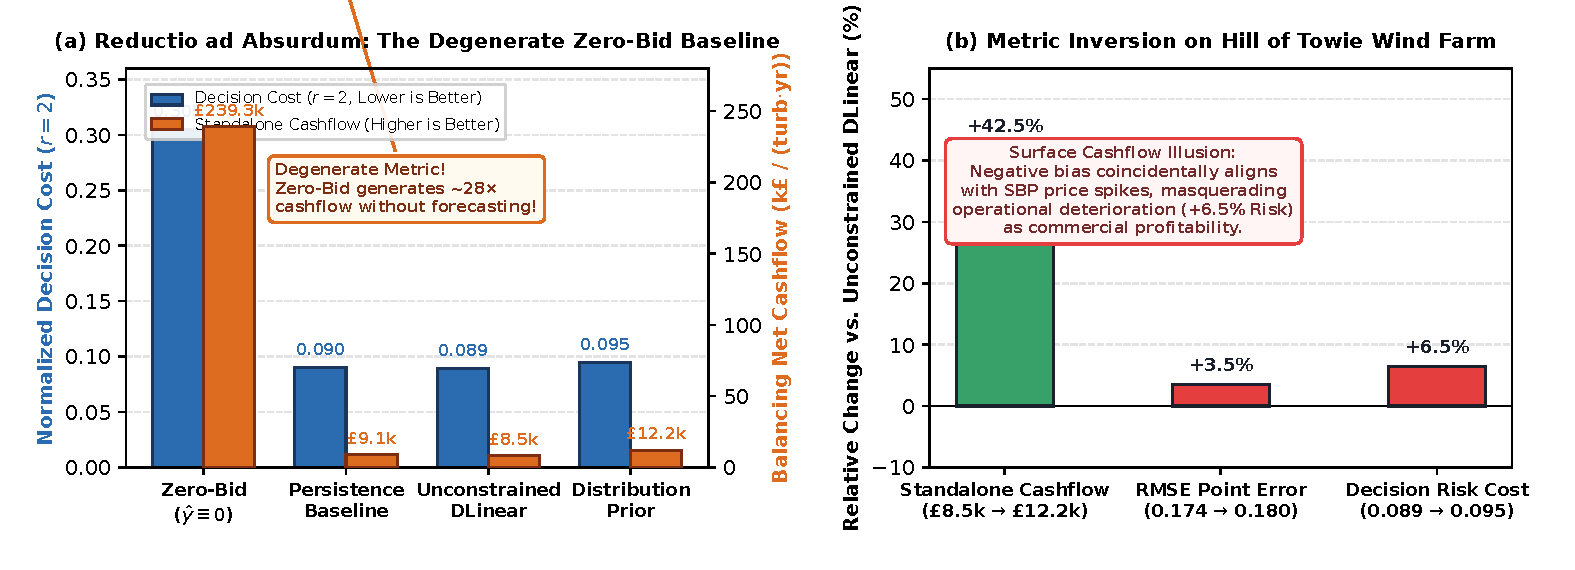
\includegraphics[width=\textwidth]{fig_market_decoupling.pdf}
\caption{Market Settlement Decoupling and Metric Inversion Diagnostic under Half-Hour Imbalance Accounting. (a) Reductio ad absurdum: the degenerate zero-bid settlement anomaly ($q \equiv 0$) incurs zero shortfall penalty and mechanically generates over \pounds 220k/turb$\cdot$yr in apparent cashflow without generating forecasts, exposing unhedged imbalance cashflow as an evaluation trap. (b) Empirical metric inversion on Hill of Towie, where distribution constraints increase nominal balancing cashflow by $+42.5\%$ while concurrently degrading genuine decision risk by $+6.5\%$ and RMSE by $+3.5\%$.}
\label{fig:market_decoupling}
\end{figure*}

Because $q \equiv 0 \le y_t$ holds almost surely for non-negative wind generation, the Zero-Bid strategy incurs exactly \textbf{\pounds 0.00 in shortfall penalties} across all three wind farms. In standalone unhedged balancing accounting, Zero-Bid mechanically generates massive apparent cashflows:
\begin{itemize}[leftmargin=*]
\item \textbf{Kelmarsh}: $+\pounds 223{,}882$/(turb$\cdot$yr);
\item \textbf{Hill of Towie}: $+\pounds 239{,}299$/(turb$\cdot$yr);
\item \textbf{Penmanshiel}: $+\pounds 243{,}450$/(turb$\cdot$yr).
\end{itemize}

We explicitly emphasize that \textbf{these six-figure sums represent uncontracted physical spill, not commercial profit or economic value}. In actual wholesale electricity markets (governed by the two-settlement identity $R_{\text{total}} = P_{\text{F}} \cdot q + P_{\text{imb}} \cdot (y - q)$ in Eq.~\eqref{eq:two_settlement}), bidding zero forfeits all forward contract revenue ($P_{\text{F}} \cdot q = 0$). When evaluated under the ground-truth asymmetric operational dispatch loss ($r=2, q=1/3$), Zero-Bid is heavily penalized, yielding normalized decision costs of $0.30409$ to $0.33689$ (matching the normalized mean capacity factor $\bar{y}$, Table~\ref{tab:zero_bid_diagnostic}).

Furthermore, on Hill of Towie, distribution regularization increases nominal balancing cashflow by $+42.5\%$ (\pounds 8,543 to \pounds 12,174/(turb$\cdot$yr); Table~\ref{tab:zero_bid_diagnostic}) while concurrently degrading normalized decision risk ($\text{Cost}_{\text{static}}$) by $+6.5\%$ and RMSE by $+3.5\%$ (Figure~\ref{fig:market_decoupling}b). This divergence occurs because the prior induces a systematic negative bias that happens to coincide with positive price spikes, creating apparent cashflow gains that mask operational dispatch degradation.

\subsection{Dynamic Market Settlement Diagnostic under 2017 UK BSC Prices}
To assess how physical constraints perform under non-stationary market conditions, we evaluated models across full-year 2017 UK Elexon BSC System Buy Prices in a stylized settlement diagnostic (Table~\ref{tab:paired_bootstrap}).

\begin{table*}[!t]
\centering
\vspace{-6pt}
\footnotesize
\renewcommand{\arraystretch}{0.80}
\setlength{\tabcolsep}{3.0pt}
\caption{7-Day Circular Block Paired Bootstrap Contrasts vs. Unconstrained DLinear under Calibrated Policy (2,000 Replications).}
\label{tab:paired_bootstrap}
\begin{threeparttable}
\begin{tabularx}{\textwidth}{p{2.2cm}p{3.2cm}>{\centering\arraybackslash}X>{\centering\arraybackslash}X>{\centering\arraybackslash}X}
\toprule
\textbf{Site} & \textbf{Method Contrast} & \textbf{Dynamic Cost Diff $\Delta \text{Cost}_{\text{dyn}}$} & \textbf{Shortfall Cashout Diff} & \textbf{Balancing Cashflow Diff} \\
 & & \textbf{(95\% CI)} & \textbf{\pounds/(turb$\cdot$yr) (95\% CI)} & \textbf{\pounds/(turb$\cdot$yr) (95\% CI)} \\
\midrule
\multirow{4}{=}{\textbf{Hill of Towie}} 
& Bounds vs.\ DLinear & $+0.000000$ ($[+0.000000, +0.000000]$) & $+\pounds 0.15$ ($[-0.17, +0.51]$) & $-\pounds 0.32$ ($[-1.37, +0.62]$) \\
& Power Curve vs.\ DLinear & $-0.000008$ ($[-0.000021, +0.000007]$) & $+\pounds 22.99$ ($[+10.93, +38.43]$) & $-\pounds 89.40$ ($[-133.51, -54.70]$) \\
& Distribution Prior vs.\ DLinear & \textbf{$+0.000766$ ($[+0.000277, +0.001201]$)} & \textbf{$-\pounds 578.57$ ($[-834.86, -367.51]$)} & \textbf{$+\pounds 1,481.27$ ($[+802.29, +2,203.32]$)} \\
& Ridge vs.\ DLinear & $-0.000733$ ($[-0.001315, -0.000125]$) & $+\pounds 192.50$ ($[-26.66, +445.74]$) & $-\pounds 1,151.96$ ($[-1,567.98, -795.28]$) \\
\midrule
\multirow{4}{=}{\textbf{Kelmarsh}} 
& Bounds vs.\ DLinear & $+0.000001$ ($[+0.000000, +0.000002]$) & $+\pounds 1.72$ ($[-0.01, +4.63]$) & $-\pounds 4.62$ ($[-12.67, +0.05]$) \\
& Power Curve vs.\ DLinear & $-0.000039$ ($[-0.000054, -0.000023]$) & $-\pounds 16.61$ ($[-33.12, +0.87]$) & $+\pounds 19.51$ ($[-27.76, +62.86]$) \\
& Distribution Prior vs.\ DLinear & \textbf{$+0.000932$ ($[+0.000423, +0.001385]$)} & \textbf{$+\pounds 932.56$ ($[+648.20, +1,236.74]$)} & \textbf{$-\pounds 3,264.86$ ($[-4,365.40, -2,223.50]$)} \\
& Ridge vs.\ DLinear & $+0.001338$ ($[+0.000917, +0.001794]$) & $+\pounds 750.61$ ($[+330.70, +1,151.06]$) & $-\pounds 690.94$ ($[-1,669.76, +409.51]$) \\
\bottomrule
\end{tabularx}
\begin{tablenotes}[flushleft]
\footnotesize
\item \textbf{Interpretation}: Negative shortfall cashout difference indicates cost reduction relative to unconstrained DLinear. Positive balancing cashflow difference indicates higher net cashflow component credited from the balancing mechanism. Confidence intervals estimated via 2,000 replications of 7-day circular block paired bootstrapping to account for temporal autocorrelation.
\end{tablenotes}
\end{threeparttable}
\end{table*}

Across dynamic settlement, physical constraints produce divergent operational outcomes across sites: on Kelmarsh, calibrated distribution constraints increase annual shortfall expenditure by \pounds 932.56/(turb$\cdot$yr) (95\% CI: $[+\pounds 648.20, +\pounds 1{,}236.74]$) and reduce net balancing cashflow by $-\pounds 3{,}264.86$/(turb$\cdot$yr). Conversely, on Hill of Towie, distribution constraints reduce annual shortfall expenditure by \pounds 578.57/(turb$\cdot$yr) and increase net balancing cashflow by \pounds 1{,}481.27/(turb$\cdot$yr) (95\% CI: $[+\pounds 802.29, +\pounds 2{,}203.32]$).

Methodologically, our framework strictly separates two orthogonal sources of empirical variation:
\begin{enumerate}[leftmargin=*]
\item \textbf{Temporal Autocorrelation Sampling Uncertainty (Delivery Period)}: The bootstrap intervals in Table~\ref{tab:paired_bootstrap} are estimated via 2,000 replications of 7-day circular block paired bootstrapping ($L=1{,}008$ steps), capturing atmospheric autocorrelation, weather regime shifts, and non-stationary price volatility.
\item \textbf{Initialization Stochasticity (Parameter Variance)}: The multi-seed dispersion metrics (mean $\pm$ standard deviation) in Table~\ref{tab:controlled_ablation} isolate parameter initialization randomness and mini-batch trajectories across identical training data.
\end{enumerate}

\subsection{Supporting Software Forensics: The Physics-Constrained Transformer}
Beyond evaluation metrics, establishing reliable empirical attribution requires verifying that executed software faithfully implements published mathematics. The Physics-Constrained Transformer (PCT \cite{pct2026}, \textit{Scientific Reports} 2026; commit \texttt{65941ec}) represents the sole publicly accessible training codebase for end-to-end physics-constrained Transformers and serves as an illustrative forensic case study.

In Section 2 of the PCT paper, the authors specify the symmetric Jensen--Shannon (JS) divergence:
\begin{equation}
\mathcal{L}_{\text{JS}}(P_{\text{pred}} \parallel P_{\text{ref}}) = \frac{1}{2} \text{KL}\left(P_{\text{pred}} \,\Big\|\, M\right) + \frac{1}{2} \text{KL}\left(P_{\text{ref}} \,\Big\|\, M\right),
\label{eq:js_divergence}
\end{equation}
where $M = \frac{1}{2}(P_{\text{pred}} + P_{\text{ref}})$.

However, static AST inspection of the official training script (\texttt{train\_clean.py}, lines 349--352) reveals that the computational graph evaluates:
\begin{equation}
\begin{split}
\mathcal{L}_{\text{code}} &= \frac{1}{2} \text{KL}\left(M \parallel P_{\text{pred}}\right) + \frac{1}{2} \text{KL}\left(M \parallel P_{\text{ref}}\right).
\end{split}
\label{eq:reverse_js}
\end{equation}
This occurs because PyTorch's \texttt{torch.nn.functional.kl\_div(input, target)} computes $\sum_i \text{target}_i (\log \text{target}_i - \text{input}_i) = \text{KL}(\text{target} \parallel \text{input})$. Passing \texttt{pred\_kde.log()} as input binds $P_{\text{pred}}$ to the denominator, executing what we designate the \textbf{reverse-argument JS form}.

Differentiating $\mathcal{L}_{\text{code}}$ directly with respect to $P_{\text{pred}, i}$ yields:
\begin{equation}
\frac{\partial \mathcal{L}_{\text{code}}}{\partial P_{\text{pred}, i}} = \frac{1}{4} \left[ \log \left(\frac{M_i^2}{P_{\text{pred}, i} P_{\text{ref}, i}}\right) + 1 - \frac{P_{\text{ref}, i}}{P_{\text{pred}, i}} \right].
\label{eq:reverse_js_gradient}
\end{equation}
Equation~\eqref{eq:reverse_js_gradient} exposes an analytical \textbf{inverse-density singularity}: whenever $P_{\text{pred}, i} \to 0$ in a region where empirical data exists ($P_{\text{ref}, i} > 0$), the ratio $\frac{P_{\text{ref}, i}}{P_{\text{pred}, i}}$ diverges as $\mathcal{O}(1/\epsilon)$. In contrast, for the mathematically specified Standard-JS in Eq.~\eqref{eq:js_divergence}, the partial derivative is bounded above by $\frac{1}{2}\ln 2 \approx 0.3466$ and exhibits only mild logarithmic divergence ($\mathcal{O}(|\log \epsilon|)$).

\begin{figure*}[!t]
\centering
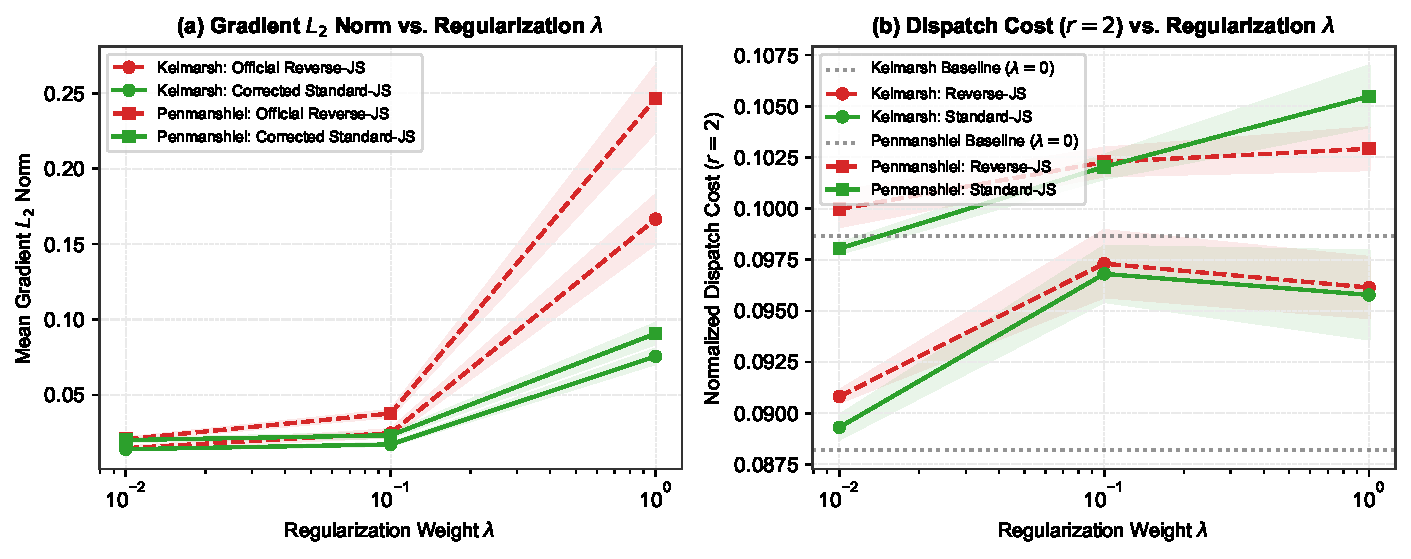
\includegraphics[width=\textwidth]{fig_pct_loss_empirical_contrast.pdf}
\caption{Empirical Optimization Contrast between Official Reverse-JS and Corrected Standard-JS on Kelmarsh and Penmanshiel. (a) Mean gradient $L_2$ norm: the reverse-argument JS form induces substantial gradient amplification at $\lambda = 1.0$ ($2.20\times$ on Kelmarsh, $2.72\times$ on Penmanshiel) due to the $-\frac{P_{\text{ref}, i}}{4 P_{\text{pred}, i}}$ singularity ($\mathcal{O}(1/\epsilon)$ in Eq.~\eqref{eq:reverse_js_gradient}). (b) Operational dispatch cost ($r=2$): Corrected Standard-JS prevents premature performance degradation at weak $\lambda=0.01$, while excessive regularization degrades dispatch across both distribution prior variants.}
\label{fig:pct_loss_empirical}
\end{figure*}

\paragraph{Empirical Gradient and Dispatch Contrast}
Empirical training on Kelmarsh and Penmanshiel across five seeds confirms that this implementation divergence materially alters optimization (Figure~\ref{fig:pct_loss_empirical}). At $\lambda = 1.0$, the reverse-argument JS form amplifies mean gradient $L_2$ norms by $2.20\times$ on Kelmarsh ($0.1665 \pm 0.0160$ vs.\ $0.0756 \pm 0.0048$) and by $2.72\times$ on Penmanshiel ($0.2465 \pm 0.0217$ vs.\ $0.0907 \pm 0.0067$; Figure~\ref{fig:pct_loss_empirical}a). At weak regularization ($\lambda = 0.01$ on Penmanshiel), Corrected Standard-JS achieves a dispatch cost of $0.09804 \pm 0.00024$, whereas the official reverse-argument implementation inflates dispatch cost to $0.09997 \pm 0.00086$ (a $+1.35\%$ degradation; Figure~\ref{fig:pct_loss_empirical}b). Under strong regularization ($\lambda = 1.0$), excessive penalization degrades operational dispatch across both distribution prior variants.

\paragraph{Negative Control: Algebraic Verification of 2D Product-Kernel KDE}
To establish an objective negative control and verify that our audit does not falsely report errors where none exist, we algebraically verified the tensor outer product $G = K_p^\top K_w \in \mathbb{R}^{B_p \times B_w}$ in the PCT codebase. Expanding the matrix product element at grid coordinate $(i,j)$ yields:
\begin{equation}
\left[ K_p^\top K_w \right]_{i,j} = \sum_{s=1}^N \phi\left( \frac{b_i^p - P_s}{h_p} \right) \cdot \phi\left( \frac{b_j^w - w_s}{h_w} \right).
\label{eq:kde_proof}
\end{equation}
Equation~\eqref{eq:kde_proof} is the exact analytical definition of a standard \textbf{paired 2D product-kernel Kernel Density Estimator} on correlated bivariate data. Because the summation contracts over concurrent sample index $s$, empirical joint coupling between wind speed and power is preserved. This confirms that software discrepancies in the audited codebase were strictly localized to the divergence argument order, rather than upstream kernel estimation.
